\documentclass{article}
\usepackage[UTF8]{ctex}
\usepackage[utf8]{inputenc} % allow utf-8 input
\usepackage[T1]{fontenc}    % use 8-bit T1 fonts
\usepackage{hyperref}       % hyperlinks
\usepackage{url}            % simple URL typesetting
\usepackage{booktabs}       % professional-quality tables
\usepackage{amsfonts}       % blackboard math symbols
\usepackage{nicefrac}       % compact symbols for 1/2, etc.
\usepackage{microtype}      % microtypography
\usepackage{lipsum}
\usepackage{geometry}
\usepackage{graphicx} %插入图片的宏包
\usepackage{float} %设置图片浮动位置的宏包
\usepackage{subfigure} %插入多图时用子图显示的宏包
\usepackage{listings}
\usepackage{soul}
\usepackage[colorlinks,linkcolor=blue]{hyperref}
\usepackage{tikz}
\usetikzlibrary{positioning, shapes.geometric}

\geometry{a4paper,scale=0.8}
\date{}

\usepackage{listings}
\usepackage{color}

\definecolor{dkgreen}{rgb}{0,0.6,0}
\definecolor{gray}{rgb}{0.5,0.5,0.5}
\definecolor{mauve}{rgb}{0.58,0,0.82}

\lstset{frame=tb,
  language=Python,
  aboveskip=3mm,
  belowskip=3mm,
  showstringspaces=false,
  columns=flexible,
  basicstyle={\small\ttfamily},
  numbers=none,
  numberstyle=\tiny\color{gray},
  keywordstyle=\color{blue},
  commentstyle=\color{dkgreen},
  stringstyle=\color{mauve},
  breaklines=true,
  breakatwhitespace=true,
  tabsize=3
}

\title{熵的性质}


\author{
Properties of the Entropy\\
 刘卓\\
 \texttt{ } \\
}

\begin{document}
\maketitle

\section{信息论的一些基本要素}

\textbf{例1}
考虑两个字母表各个字符的概率:

$$
\begin{array}{|l|l|l|l|l|}
\hline
\mbox{字母}&A&B&C&D\\
\hline
\mbox{字母表1的频数}&\frac{1}{4}&\frac{1}{4}&\frac{1}{4}&\frac{1}{4}\\
\hline
\mbox{字母表2的频数}&\frac{1}{2}&\frac{1}{4}&\frac{1}{8}&\frac{1}{8}\\
\hline
\end{array}
$$

请问多少个\textbf{是/否(Yes or No)问题}可以判断出每一个字母?

~\\

解:

字母表1判断方法:

$$
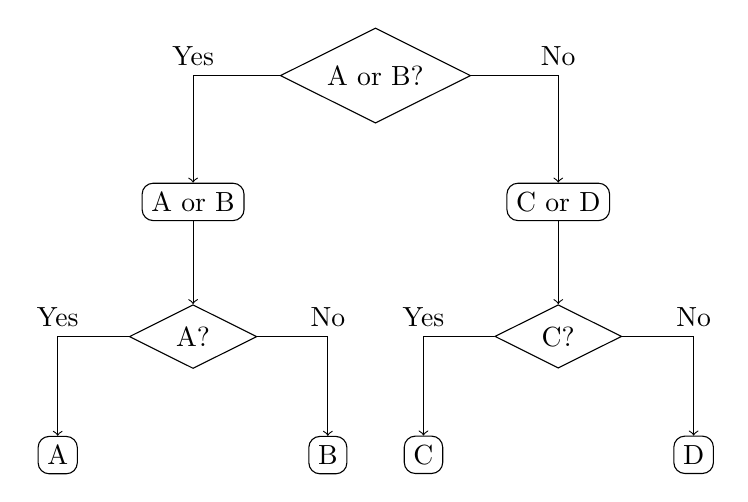
\begin{tikzpicture}[node distance=10pt]
  \node[draw, diamond, aspect=2]     (AB)  {A or B?};
  \node[draw, rounded corners, aspect=2,  below left=30pt and 30pt of AB]     (1A)  {A or B};
  \node[draw, rounded corners, aspect=2,  below right=30pt and 30pt of AB]     (1C)  {C or D};
  \node[draw, diamond, aspect=2, below=30pt of 1A]     (2A)  {A?};
  \node[draw, diamond, aspect=2, below=30pt of 1C]     (2C)  {C?};
  \node[draw, rounded corners, aspect=2,  below left=30pt and 30pt of 2A]     (3A)  {A};
  \node[draw, rounded corners, aspect=2,  below right=30pt and 30pt of 2A]     (3B)  {B};
  \node[draw, rounded corners, aspect=2,  below left=30pt and 30pt of 2C]     (3C)  {C};
  \node[draw, rounded corners, aspect=2,  below right=30pt and 30pt of 2C]     (3D)  {D};
  
  \draw[->] (AB) -| node[above]  {Yes} (1A);
  \draw[->] (AB) -| node[above]  {No} (1C);
  \draw[->] (1A) --  (2A);
  \draw[->] (1C) --  (2C);
  \draw[->] (2A) -| node[above]  {Yes} (3A);
  \draw[->] (2A) -| node[above]  {No} (3B);
  \draw[->] (2C) -| node[above]  {Yes} (3C);
  \draw[->] (2C) -| node[above]  {No} (3D);
\end{tikzpicture}
$$

平均需要$\color{red}{2}$次询问才可以确定一个字符;

~\\

字母表2判断方法:

$$
\begin{tikzpicture}[node distance=10pt]
  \node[draw, diamond, aspect=2]     (A?)  {A?};
  \node[draw, below right=30pt  and 30pt of A?]                   (step x)  {B,C,or D};
  \node[draw, rounded corners, below left=30pt and 30pt of A?]  (A)     {A};
  \node[draw, diamond, aspect=2, below=30pt of step x]     (2)  {B?};
  \node[draw, rounded corners, aspect=2,  below left=30pt and 30pt of 2]     (3)  {B};
  \node[draw, rounded corners, aspect=2,  below right=30pt and 30pt of 2]     (4)  {C or D};
  \node[draw, diamond, aspect=2, below=30pt of 4]     (5)  {C?};
  \node[draw, rounded corners, aspect=2,  below left=30pt and 30pt of 5]     (6)  {C};
  \node[draw, rounded corners, aspect=2,  below right=30pt and 30pt of 5]     (7)  {D};
  

  \draw[->] (A?) -| node[above]  {Yes} (A);
  \draw[->] (A?) -| node[above] {No}  (step x);
  \draw[->] (step x) --  (2);
  \draw[->] (4) --  (5);
  \draw[->] (2) -| node[above]  {Yes} (3);
  \draw[->] (2) -| node[above]  {No} (4);
  \draw[->] (5) -| node[above]  {Yes} (6);
  \draw[->] (5) -| node[above]  {No} (7);
\end{tikzpicture}
$$

平均需要$\underbrace{1 \cdot \frac{1}{2}}_{A}+\underbrace{2 \cdot \frac{1}{4}}_{B}+\underbrace{3 \cdot \frac{1}{4}}_{C}+\underbrace{3 \cdot \frac{1}{4}}_{D} = \color{red}{1.75}$次询问就可以确定一个字符;
$\quad\quad\quad\quad\quad\quad\quad\quad\quad\quad\quad\quad\quad\quad\quad\quad\quad\quad\quad\quad\quad\quad\quad\quad\quad\quad\quad\quad\quad\Box$


~\\

用$1$代表$\color{green}{Yes}$, $0$代表$\color{red}{No}$。就可以使用一个二进制数字表示是/否问题的结果。一般来说,如果实验有N个可能的\textbf{均等}结果,那么需要:
$$log_2(N)$$
信息大小(bit)以存储实验结果。

\textbf{例2}
\begin{enumerate}
\item 一个六面色子,需要$log_2(6) \approx 2.585$bit单位。向上取整,需要3个bit来储存信息。
\item 拉丁字母表,需要$log_2(26) \approx4.7$bit单位。向上取整,需要5个bit来储存信息。
\item ASCII表,需要$log_2(128) =7$bit单位来储存信息。
\end{enumerate}


~\\

如果实验结果是的\textbf{不均等}的。如果事件A发生概率为$p=\mathbb{P}[Z=A]$,那么每个字符需要大小为
$$log_2(\frac{1}{p})$$
的储存空间。

所有事件合在一起所需要的空间一共是:
$$\sum_a p\cdot log_2{\frac{1}{p}}$$

\textit{定义1:事件A的熵是对我们对事件A发生的不确定性的度量。随机变量X的熵为
$$
H(X)=\sum_{a} \mathbb{P}(X=a) \cdot \log _{2}\left(\frac{1}{\mathbb{P}(X=a)}\right)
$$
}

\textit{定义2:两个随机变量X和Y的熵为
$$
H(X, Y)=\sum_{a, b} \mathbb{P}(X=a, Y=b) \cdot \log _{2}\left(\frac{1}{\mathbb{P}(X=a, Y=b)}\right)
$$
}

\textit{定义3:如果\textbf{事件Y}发生,随机变量X的条件熵为
$$
H(X|Y)=\sum_{a} \mathbb{P}(X=a|Y) \cdot \log _{2}\left(\frac{1}{\mathbb{P}(X=a|Y)}\right)
$$
}

\textit{定义4:给定\textbf{随机变量Y}的随机变量X的条件熵为
$$
H(X|Y)=\sum_{b} \mathbb{P}(Y=b) \cdot \ H(X|Y=b))
$$
}


\textbf{例3}

如图所示,假设随机变量X,Y,Z是通过旋转获得的。
其中X由\textbf{最里面}的圆给定的,Y由\textbf{中间圆}给定的
,Z由\textbf{最外面}的圆给定的。

\begin{figure}[H] %H为当前位置,!htb为忽略美学标准,htbp为浮动图形
\centering %图片居中
\includegraphics[width=0.5\textwidth]{图库/9.1.png} %插入图片,[]中设置图片大小,{}中是图片文件名
\label{Fig.main2} %用于文内引用的标签
\end{figure}

(1)计算$H(X)$

$$
\begin{array}{|l|l|l|l|l|}
\hline
a&-1&0&1&3\\
\hline
P(X=a)&\frac{1}{4}&\frac{3}{8}&\frac{1}{4}&\frac{1}{8}\\
\hline
\end{array}
$$

$$H(X) = \frac{1}{4} \cdot log_2(\frac{1}{1/4})+\frac{3}{8} \cdot log_2(\frac{1}{3/8})+\frac{1}{4} \cdot log_2(\frac{1}{1/4})+\frac{1}{8} \cdot log_2(\frac{1}{1/8}) \approx 1.906$$

(2)需要多少bit来存储结果100,000次Z旋转?

$$
\begin{array}{|l|l|l|l|}
\hline
a&1&2&3\\
\hline
P(Z=a)&\frac{1}{3}&\frac{1}{3}&\frac{1}{3}\\
\hline
\end{array}
$$

$$H(Z) = \frac{1}{3} \cdot log_2(\frac{1}{1/3})+\frac{1}{3} \cdot log_2(\frac{1}{1/3})+\frac{1}{3} \cdot log_2(\frac{1}{1/3})= log_2(3) \approx 1.585$$


$$H(Z) \cdot 100000 =158500 \ bit $$

(3)给定X = 0,计算Z的熵

$$H(Z|X=0)=\sum_a P(Z=a|X=0) \cdot \ log_2(\frac{1}{P(Z=a|X=0)})=\frac{2}{3}\cdot log_2(\frac{2}{3})+\frac{1}{3}\cdot log_2(\frac{1}{3}) \approx 0.9183$$

(4)计算$H(Z|Y)$

$$H(Z|Y) = \sum_y P(Y=y) \cdot H(Z|Y=y)=\frac{3}{8} \cdot H(Z|Y=-1)+\frac{3}{8} \cdot H(Z|Y=1)+\frac{1}{4}\cdot H(Z|Y=0)$$

$H(Z|Y=y)$计算方法同上;

~\\

\textbf{注意}:如果X,Y是不相关的(independent),那么$H(Y|X)=H(Y)$

~\\

(5)计算$H(X|Y,Z)$

$H(X|Y,Z) = 0$如果X可以用Y,Z代替。即:一旦$X=aY^n+bZ^m$,n,m为整数,那么$H(X|Y,Z) = 0$。本题满足该条件。





~\\

假设我们知道X的值,然后知道Y的值,则
$$H(X,Y) = H(X)+H(Y|X)$$

$$H(X_1,X_2,\cdots,X_n) = H(X_1)+H(X_2|X_1)+H(X_3|X_1,X_2)+\cdots+H(X_n|X_1,X_2,\cdots,X_{n-1})$$

\href{http://www.cs.tau.ac.il/~iftachh/Courses/Info/Fall14/Printouts/Lesson2_h.pdf}{\color{blue}{证明过程请参考这里}}

$\quad\quad\quad\quad\quad\quad\quad\quad\quad\quad\quad\quad\quad\quad\quad\quad\quad\quad\quad\quad\quad\quad\quad\quad\quad\quad\quad\quad\quad\quad\quad\quad\quad\quad\quad\quad\quad\quad\quad\Box$

\section*{一些重要不等式}

1. 对于仅取$k$个值的随机变量$X$,总是满足:
$$H(X) \leq log_2(k)$$

当且仅当X以相等的概率取其所有值时才相等。

~\\

证明:


\begin{eqnarray}   
\label{eq}
H(X)&=& \sum \mathbb{P}(X=a) \cdot \log_2(\frac{1}{\mathbb{P}(X=a)}) \nonumber \\ 
&\leq& \log_2 (\sum \mathbb{P}(X=a) \cdot \frac{1}{\mathbb{P}(X=a)}) \ \nonumber \\ 
&=& \log_2(k) \nonumber \\ 
\nonumber 
\end{eqnarray}


~\\

2.对于两个随便变量$X$和$Y$来说,总是满足:

$$H(X,Y) \leq H(X) + H(Y)$$

当且仅当$X$和$Y$是不相关(independent)时,等式成立。

~\\

证明:
$$H(X|Y) H(X) + H(Y|X )\leq H(X) + H(Y)$$


~\\

3.对于两个随便变量$X$和$Y$来说,总是满足:

$$H(X|Y) \leq H(X)$$

当且仅当$X$和$Y$是不相关(independent)时,等式成立。

~\\

证明:


\begin{eqnarray}   
\label{eq}
H(X,Y)&=& \sum_b \mathbb{P}(Y=b)H(X|Y=b)\nonumber \\ 
&=&\sum_b \mathbb{P}(Y=b) \sum_a \mathbb{P}(X=a|Y=b) \log_2 \left( \frac{1}{\mathbb{P}(X=a|Y=b)} \right)  \nonumber \\  
&=&  \sum_b \mathbb{P}(Y=b) \sum_a \frac{\mathbb{P}(X=a \cap Y=b)}{\mathbb{P}(Y=b)} \times \log_2 \left( \frac{1}{\mathbb{P}(X=a|Y=b)} \right) \nonumber \\  
&=& \sum_b \sum_a \mathbb{P}(X=a \cap Y=b) \log_2 \left( \frac{1}{\mathbb{P}(X=a|Y=b)} \right)\nonumber \\  
&=& \sum_a \mathbb{P}(X=a) \sum_b \frac{\mathbb{P}(Y=b \cap X=a )}{\mathbb{P}(X=a)}  \log_2 \left( \frac{1}{\mathbb{P}(X=a|Y=b)} \right)\nonumber \\  
&=& \sum_a \mathbb{P}(X=a) \sum_b\mathbb{P}( Y=b|X=a )  \log_2 \left( \frac{1}{\mathbb{P}(X=a|Y=b)} \right)\nonumber \\  
&\leq&  \sum_a \mathbb{P}(X=a) \log_2 \left(  \sum_b \frac{\mathbb{P}(X=a|Y=b)} {\mathbb{P}(X=a|Y=b)} \right)\nonumber \\  
&=&\sum_a \mathbb{P}(X=a) \log_2 \left(  \sum_b \frac{\mathbb{P}(Y=b \cap X=a)} {\mathbb{P}(X=a)} \times \frac{\mathbb{P}(Y=b)} {\mathbb{P}(X=a \cap Y=b)} \right)\nonumber \\
&=& \sum_a \mathbb{P}(X=a) \log_2 \left(  \sum_b \frac{\mathbb{P}(Y=b)} {\mathbb{P}(X=a)} \right)\nonumber \\
&=& \sum_a \mathbb{P}(X=a) \log_2 \left( \frac{\1} {\mathbb{P}(X=a)} \right) \nonumber \\
&=& H(X)\nonumber \\
\nonumber 
\end{eqnarray}

\section{英语中的熵}

以下是英文写作中大约1000个字母频率表:

$$
&\begin{array}{|c|c|c|c|c|c|c|c|c|c|c|c|c|c|}
\hline \text { \mbox{字母} } & \text { a } & \text { b } & \text { c } & \text { d } & \text { e } & \text { f } & \text { g } & \text { h } & \text { i } & \text { j } & \text { k } & \text { l } & \text { m } \\
\hline \text {\mbox{频数} } & 73 & 9 & 30 & 44 & 130 & 28 & 16 & 35 & 74 & 2 & 3 & 35 & 25 \\
\hline
\end{array}\\
$$
$$
&\begin{array}{|c|c|c|c|c|c|c|c|c|c|c|c|c|}
\hline \mathrm{n} & \mathrm{o} & \mathrm{p} & \mathrm{q} & \mathrm{r} & \mathrm{s} & \mathrm{t} & \mathrm{u} & \mathrm{v} & \mathrm{w} & \mathrm{x} & \mathrm{y} & \mathrm{z} \\
\hline 78 & 74 & 27 & 3 & 77 & 63 & 93 & 27 & 13 & 16 & 5 & 19 & 1 \\
\hline
\end{array}
$$

计算英语中的熵公式为:

\begin{eqnarray}   
\label{eq}
H(X)&=&\sum_{\alpha=A}^{Z} \mathbb{P}[X=\alpha] \cdot \log _{2}\left(\frac{1}{\mathbb{P}[X=\alpha]}\right)\nonumber \\ 
&=&\mathbb{P}(A) \log_2 \left(  \frac{1}{\mathbb{P}(A)}\right) + \cdots + \mathbb{P}(Z) \log_2 \left(  \frac{1}{\mathbb{P}(Z)}\right)\nonumber \\
&=& 0.073 \cdot  \log_2 \left(  \frac{1}{0.073}\right)+ \cdots + 0.001\cdot  \log_2 \left(  \frac{1}{0.001}\right) \nonumber \\
&\approx & 4.1621 \nonumber \\
\nonumber 
\end{eqnarray}

移位平均需要4.1621个bit来储存一个拉丁字母。

\section{摩斯密码}

摩斯密码(Morse code)是一种时通时断的信号代码
通过不同的排列顺序来表达不同的英文字母、数字和标点符号。是由美国人艾尔菲德·维尔与萨缪尔·摩尔斯在1836年发明。

\begin{enumerate}
\item 点( · ):1 (读 “滴” dit ,时间占据1t )
\item 划(—):111 (读 “嗒” dah ,时间占据3t )
\item 字符内部的停顿(在点和划之间):0 (时间占据1t )
\item 字符间停顿:000 ( 时间占据3t )
\item 单词间的停顿:0000000 ( 时间占据7t )
\end{enumerate}

点的长度(也就是上面的时间长度t)决定了发报的速度。

\begin{figure}[H] %H为当前位置,!htb为忽略美学标准,htbp为浮动图形
\centering %图片居中
\includegraphics[width=0.7\textwidth]{图库/res07_attpic_brief.jpg} %插入图片,[]中设置图片大小,{}中是图片文件名
\caption{国际摩斯密码} %最终文档中希望显示的图片标题
\label{Fig.main2} %用于文内引用的标签
\end{figure}

其熵约为: 7.039,意味着平均需要7个bit来储存一个字符。

\end{document}

